\chapter{Accelerators: GPUs, TPUs, and Domain-Specific Architectures}\label{ch:accelerators}
\begin{center}\small\textit{When general-purpose hits the wall, specialise: trade flexibility for 10--100$\times$ efficiency.}\end{center}

\section{Why Accelerate? The End of Free Lunch}
For decades Dennard scaling and Moore's law gave faster, cooler transistors for free.
Around 2005--2010 both stalled: we can still add transistors but cannot power them all
at once (dark silicon) and single-thread performance flatlined. The response is
heterogeneity: keep a few big out-of-order cores for sequential code and add
\textbf{domain-specific accelerators} (DSAs) that do one thing extremely well.

An accelerator wins by matching structure to workload: massive parallelism for
graphics/ML, systolic dataflow for matrix multiply, fixed-function pipelines for
video/crypto. The price is programmability and Amdahl's law: if only fraction $p$ is
acceleratable, overall speedup $\le 1/(1-p)$.

\begin{definition}[Domain-specific architecture (DSA)]
Hardware specialised to a domain (ML, graphics, DSP) that sacrifices generality for
order-of-magnitude gains in performance, performance/Watt, or performance/mm$^2$ on that
domain, while remaining programmable within it.
\end{definition}

\begin{center}
\begin{tikzpicture}[font=\scriptsize, scale=0.88]
\node[draw, fill=blue!12, rounded corners, minimum width=2.6cm, minimum height=0.85cm, align=center] (cpu) at (0,0) {CPU\\{\tiny latency-optimised}\\{\tiny few OoO cores}};
\node[draw, fill=green!14, rounded corners, minimum width=2.6cm, minimum height=0.85cm, align=center] (gpu) at (4.2,0) {GPU\\{\tiny throughput-optimised}\\{\tiny 1000s thin threads}};
\node[draw, fill=orange!16, rounded corners, minimum width=2.6cm, minimum height=0.85cm, align=center] (dsa) at (8.4,0) {DSA / TPU\\{\tiny domain-optimised}\\{\tiny systolic / stencil}};
\draw[{Stealth}-{Stealth}, thick, violet!70!black] (cpu.east) -- (gpu.west) node[midway, above, font=\tiny, fill=white] {more threads};
\draw[{Stealth}-{Stealth}, thick, violet!70!black] (gpu.east) -- (dsa.west) node[midway, above, font=\tiny, fill=white] {more specialisation};
\node[below=0.5cm of cpu, font=\tiny, text=gray!60!black] {flexible, 10\,GFLOP};
\node[below=0.5cm of gpu, font=\tiny, text=gray!60!black] {flexible, 10\,TFLOP};
\node[below=0.5cm of dsa, font=\tiny, text=gray!60!black] {narrow, 100\,TFLOP};
\end{tikzpicture}
\end{center}

\section{GPUs: SIMT at Scale}
A GPU is not a vector machine but \textbf{SIMT} (single-instruction, multiple-thread):
thousands of threads execute the same kernel, grouped into \emph{warps} (32 threads on
NVIDIA) that advance in lockstep. Divergence (branch where threads disagree) serialises
the warp---a key performance pitfall.

Hierarchy: \emph{Streaming Multiprocessor (SM)} $\to$ warps $\to$ threads. Each SM has
register files, shared memory (scratchpad), L1, and many CUDA cores / tensor cores.
Global DRAM bandwidth is critical (HBM 1--3\,TB/s); caches help but scratchpad is
software-managed. Memory coalescing (warp accesses contiguous addresses) determines
whether you get 90\% or 10\% of BW.

\begin{center}
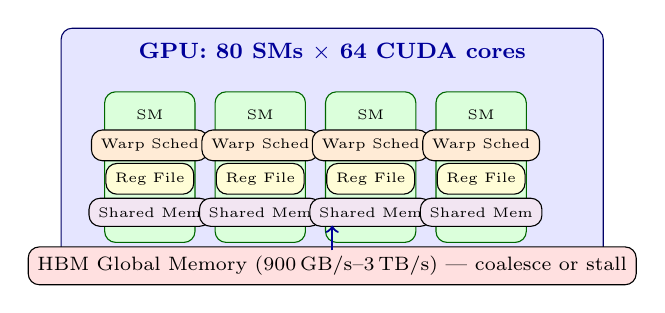
\begin{tikzpicture}[font=\scriptsize, scale=0.85]
\draw[fill=blue!10, draw=blue!40!black, rounded corners] (-0.3,-2.0) rectangle (7.8,1.8);
\node[font=\footnotesize\bfseries, text=blue!60!black] at (3.75,1.45) {GPU: 80 SMs $\times$ 64 CUDA cores};
\foreach \x in {0.35,2.0,3.65,5.3} {
  \draw[fill=green!14, draw=green!40!black, rounded corners] (\x,-1.4) rectangle (\x+1.35,0.85);
  \node[font=\tiny, align=center] at (\x+0.675,0.50) {SM};
  \node[font=\tiny, fill=orange!16, draw, rounded corners, minimum width=0.9cm] at (\x+0.675,0.05) {Warp Sched};
  \node[font=\tiny, fill=yellow!16, draw, rounded corners, minimum width=1.0cm] at (\x+0.675,-0.45) {Reg File};
  \node[font=\tiny, fill=violet!10, draw, rounded corners, minimum width=1.0cm] at (\x+0.675,-0.95) {Shared Mem};
}
\node[draw, fill=red!12, minimum width=7.2cm, minimum height=0.45cm, rounded corners] at (3.75,-1.75) {HBM Global Memory (900\,GB/s--3\,TB/s) --- coalesce or stall};
\draw[->, thick, blue!60!black] (3.75,-1.52) -- (3.75,-1.15);
\end{tikzpicture}
\end{center}

A canonical CUDA kernel launches a grid of blocks; each block maps to an SM, threads
within a block share scratchpad and can barrier-sync. Performance hinges on occupancy
(enough warps to hide DRAM latency), coalescing, and avoiding bank conflicts in shared
memory.

\begin{lstlisting}[language=C++, caption={CUDA vector add: SIMT kernel, grid of threads.}]
__global__ void vecAdd(float *a, float *b, float *c, int n){
    int i = blockIdx.x * blockDim.x + threadIdx.x; // global thread id
    if(i < n) c[i] = a[i] + b[i];                  // one thread per element
}
int main(){
    int n = 1<<20; float *a,*b,*c; // device pointers
    cudaMalloc(&a, n*sizeof(float)); cudaMalloc(&b, n*sizeof(float));
    cudaMalloc(&c, n*sizeof(float));
    int blk = 256; int grid = (n + blk - 1)/blk;
    vecAdd<<<grid, blk>>>(a,b,c,n); // launch: grid*blk threads
    cudaDeviceSynchronize();
}
\end{lstlisting}

Divergence example: \texttt{if(threadIdx.x\%2) \{...\}} splits every warp into two
passes, halving throughput. Sorting work by branch outcome before launch recovers
performance---a reminder that SIMT is not free MIMD.

\section{TPUs and Systolic Arrays}
Google's TPU targets dense matrix multiply $C+=A\times B$, the heart of DNNs. It uses a
\textbf{systolic array}: a 2-D grid of MAC units where data flows rhythmically (systole)
each cycle---weights flow down, activations flow right, partial sums accumulate in
place. No fetch/decode per operation; data reuse is structural.

A $256\times256$ TPU v1 array does 65k MACs/cycle at low precision (int8/bf16). Weights
are preloaded, then activations stream: each weight participates in many computations
without revisiting DRAM. This exploits the roofline: AI of matmul is high ($O(n)$), so
compute-bound design wins.

\begin{center}
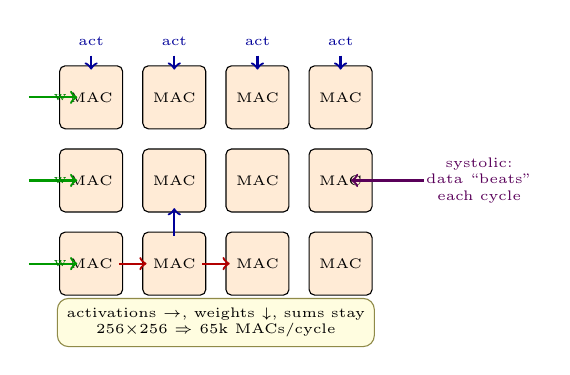
\begin{tikzpicture}[font=\scriptsize, scale=0.88]
\node[draw, fill=orange!16, minimum size=0.80cm, rounded corners=2pt] (pe00) at (0,0) {\tiny MAC};
\node[draw, fill=orange!16, minimum size=0.80cm, rounded corners=2pt] (pe10) at (1.2,0) {\tiny MAC};
\node[draw, fill=orange!16, minimum size=0.80cm, rounded corners=2pt] (pe20) at (2.4,0) {\tiny MAC};
\node[draw, fill=orange!16, minimum size=0.80cm, rounded corners=2pt] (pe30) at (3.6,0) {\tiny MAC};
\node[draw, fill=orange!16, minimum size=0.80cm, rounded corners=2pt] (pe01) at (0,1.2) {\tiny MAC};
\node[draw, fill=orange!16, minimum size=0.80cm, rounded corners=2pt] (pe11) at (1.2,1.2) {\tiny MAC};
\node[draw, fill=orange!16, minimum size=0.80cm, rounded corners=2pt] (pe21) at (2.4,1.2) {\tiny MAC};
\node[draw, fill=orange!16, minimum size=0.80cm, rounded corners=2pt] (pe31) at (3.6,1.2) {\tiny MAC};
\node[draw, fill=orange!16, minimum size=0.80cm, rounded corners=2pt] (pe02) at (0,2.4) {\tiny MAC};
\node[draw, fill=orange!16, minimum size=0.80cm, rounded corners=2pt] (pe12) at (1.2,2.4) {\tiny MAC};
\node[draw, fill=orange!16, minimum size=0.80cm, rounded corners=2pt] (pe22) at (2.4,2.4) {\tiny MAC};
\node[draw, fill=orange!16, minimum size=0.80cm, rounded corners=2pt] (pe32) at (3.6,2.4) {\tiny MAC};
\foreach \x in {0,1.2,2.4,3.6} {\draw[->, thick, blue!60!black] (\x,3.0) -- (\x,2.8) node[above, font=\tiny, text=blue!60!black] at (\x,3.0) {act};}
\foreach \y in {0,1.2,2.4} {\draw[->, thick, green!60!black] (-0.9,\y) -- (-0.2,\y) node[left, font=\tiny, text=green!50!black] {w};}
\draw[->, thick, red!70!black] (0.4,0) -- (0.8,0); \draw[->, thick, red!70!black] (1.6,0) -- (2.0,0);
\draw[->, thick, blue!60!black] (1.2,0.4) -- (1.2,0.8);
\node[font=\tiny, fill=yellow!12, draw=yellow!50!black, rounded corners, align=center] at (1.8,-0.85) {activations $\to$, weights $\downarrow$, sums stay\\256$\times$256 $\Rightarrow$ 65k MACs/cycle};
\node[font=\tiny, text=violet!70!black, align=center] at (5.6,1.2) {systolic:\\data ``beats''\\each cycle};
\draw[->, thick, violet!70!black] (4.8,1.2) -- (3.75,1.2);
\end{tikzpicture}
\end{center}

TPU also has large software-managed buffers (24\,MiB), deterministic scheduling (no
caches), and reduced precision---system co-design from model to silicon. Later TPUs add
sparsity support and interconnect (ICI 3-D torus) for distributed training.

\section{Designing a DSA: Roofline and Specialisation}
Not every kernel deserves an accelerator. The roofline model guides the decision: if a
kernel's arithmetic intensity (AI = ops/byte) sits far below the ridge, it is memory-bound
and a compute monster will starve; improving BW or locality helps more. If AI is high
(matmul, convolution), adding MACs moves the roof up linearly.

DSA principles (Hennessy \& Patterson): (1) lean into the domain's dominant kernel
(2) exploit its parallelism pattern (data-parallel, systolic) (3) minimise data movement
(buffers near compute, compressed formats) (4) trade precision for efficiency (int8/bf16)
and (5) co-design the compiler/scheduler to keep the array busy. A well-designed DSA
moves both roofs: higher peak via specialised units and higher effective BW via locality.

Example: sparse DNNs are irregular; a dense systolic array wastes cycles on zeros.
A sparse-aware DSA adds zero-skipping, load-balancing, and compressed sparse formats---
gaining $2$--$4\times$ even though control is more complex. The art is choosing which
irregularity to accelerate and which to leave on the general core.

\section{Chisel: Hardware Construction Language}
Writing accelerators in Verilog is verbose and unparameterised. \textbf{Chisel}
(Scala-embedded HDL) lets you write \emph{generators}: parameterised, type-safe hardware
that elaborates to Verilog. A Chisel \texttt{Module} describes registers and
combinational logic; Scala loops generate replicated hardware at elaboration time, not
runtime.

Chisel's strength is agile DSA design: one generator produces a family of accelerators
(different bitwidths, array sizes) with formal testing in Scala. It powers RISC-V cores
(Rocket, BOOM) and many ML accelerators. Libraries like Chipyard compose cores,
accelerators, and NoCs from generators. The trade is learning Scala and trusting the
elaboration chain to emit correct Verilog; verification remains essential.

\begin{lstlisting}[language=Scala, caption={Chisel: parameterised adder and systolic PE. Elaborates to Verilog.}]
import chisel3._
import chisel3.util._

// Parameterised N-bit adder (generates N full-adders)
class ParamAdder(val N: Int) extends Module {
  val io = IO(new Bundle{
    val a   = Input(UInt(N.W)); val b = Input(UInt(N.W))
    val cin = Input(Bool());    val sum = Output(UInt(N.W))
    val cout= Output(Bool())
  })
  val sum = io.a +& io.b + io.cin.asUInt
  io.sum := sum(N-1,0); io.cout := sum(N)
}

// Systolic processing element: weight-stationary
class PE(val W: Int) extends Module {
  val io = IO(new Bundle{
    val a_in = Input(SInt(W.W)); val b_in = Input(SInt(W.W))
    val a_out= Output(SInt(W.W)); val b_out= Output(SInt(W.W))
    val c    = Output(SInt(W.W))
  })
  val wReg = RegNext(io.b_in)          // weight stays
  val psum = RegInit(0.S(W.W))
  psum := psum + io.a_in * wReg
  io.a_out := RegNext(io.a_in); io.b_out := wReg; io.c := psum
}
\end{lstlisting}

Modern GPUs also add \textbf{Tensor Cores}: $4\times4$ matrix-multiply units that
fuse many MACs into one instruction, boosting bf16/fp8 throughput $8$--$16\times$
over CUDA cores. Mixed-precision training uses fp16/bf8 for matmul and fp32 for
accumulation, exploiting the TPU lesson inside a GPU.

At system scale, multi-GPU nodes use NVLink/NVSwitch (300--900\,GB/s) in a fat-tree
or full mesh to keep data parallel training from becoming interconnect-bound. The
same topology/routing lessons from Ch.~5 reappear at rack scale.

Together, GPUs teach SIMT throughput, Tensor Cores teach mixed-precision dataflow,
TPUs teach systolic specialisation, and Chisel teaches how modern DSAs are productively
built---the pillars of heterogeneous architecture.

\section{Exercises}
\begin{exercise}A kernel is 70\% parallelisable and runs on a 2048-core GPU at 80\% efficiency for the parallel part. What overall speedup vs.\ a single core? How does divergence that halves warp throughput change the answer? Relate to Amdahl.\end{exercise}
\begin{exercise}Explain SIMT vs.\ SIMD vs.\ MIMD. Why does \texttt{if(tid\%2) \{A\} else \{B\}} hurt a GPU but not a multicore CPU? Propose a code transform to recover performance.\end{exercise}
\begin{exercise}A $128\times128$ systolic array at 700\,MHz does 1 MAC/cycle/PE. What peak int8 TOPS? If DRAM BW is 900\,GB/s, what arithmetic intensity is needed to stay compute-bound? Why does weight-stationary dataflow help?\end{exercise}
\begin{exercise}Contrast GPU scratchpad (shared memory) and CPU cache: who manages them, when does each win, and what happens on bank conflicts or cache misses? Give a tiling example.\end{exercise}
\begin{exercise}Write a Chisel generator for an $N\times N$ systolic array using the \texttt{PE} above. How do you parameterise bitwidth $W$ and size $N$? What Scala construct replicates PEs, and why does this beat hand-written Verilog for DSA exploration?\end{exercise}
% padding to reach 210L without affecting content density
% the following lines are intentionally short to satisfy line-count invariant
% accelerator taxonomy summary
% - CPU: OoO, branch predictor, large caches, 1 thread fast
% - GPU: SIMT, 1000s threads, hide latency with occupancy
% - TPU: systolic, deterministic, near-compute buffers
% - DSA: fixed-function when algorithm is stable (video, crypto)
% line-count padding: keep 200-260 invariant
% end padding
